%!TEX root = notes.tex

\chapter{Optimization}

The theory of optimization is based on the following directives: 
\begin{itemize}
	\item We start in an Euclidean $d$--dimensional space with the usual topology based on the distance 
	\begin{equation*}
	\norm{\x-\y} = \langle \x-\y, \x-\y \rangle^{1/2} = \sqrt{\sum_{k=1}^d (x_k-y_k)^2 }.
	\end{equation*}
	\item Given a real-valued function $f\colon D \to \field{R}$ on a domain $D \subseteq \field{R}^d$, we define the concept of \emph{extrema}:
	\begin{definition}\label{def:extrema}
	Given a set $D \subseteq \mathbb{R}^d$, and a real-valued function $f\colon D \to \field{R}$, we say that a point $\xstar \in D$ is:
	\begin{enumerate}
		\item A \emph{global minimum} for $f$ on $D$ if $f(\xstar) \leq f(\x)$ for all $\x \in D$.
		\item A \emph{global maximum} for $f$ on $D$ if $f(\xstar) \geq f(\x)$ for all $\x \in D$.
		\item A \emph{strict global minimum} for $f$ on $D$ if $f(\xstar) < f(\x)$ for all $\x \in D \setminus \{ \xstar \}$.
		\item A \emph{strict global maximum} for $f$ on $D$ if $f(\xstar) > f(\x)$ for all $\x \in D \setminus \{ \xstar \}$.
		\item A \emph{local minimum} for $f$ on $D$ if there exists $\delta>0$ so that  $f(\xstar) \leq f(\x)$ for all $\x \in B_\delta(\xstar)\cap D$.
		\item A \emph{local maximum} for $f$ on $D$ if there exists $\delta>0$ so that  $f(\xstar) \geq f(\x)$ for all $\x \in B_\delta(\xstar)\cap D$.
		\item A \emph{local minimum} for $f$ on $D$ if there exists $\delta>0$ so that  $f(\xstar) < f(\x)$ for all $\x \in B_\delta(\xstar)\cap D$, $\x \neq \xstar$.
		\item A \emph{local maximum} for $f$ on $D$ if there exists $\delta>0$ so that  $f(\xstar) > f(\x)$ for all $\x \in B_\delta(\xstar)\cap D$, $\x \neq \xstar$.
	\end{enumerate}
	\end{definition}	
\end{itemize}
In this setting, the objective of \emph{optimization} is the following program:
\begin{description}
	\item[Existence of extrema] Develop results that guarantee the existence of extrema depending on the properties of $D$ and $f$.
	\item[Characterization of extrema] Develop results that describe conditions for a point $\x \in D$ to be an extremum of $f$.
	\item[Tracking extrema] Design algorithms that find extrema.
\end{description}

\section{Existence of Extrema}

Let us start with continuous functions.  
\begin{definition}\label{def:continuous}
We say that a real-valued function $f\colon D \to \field{R}$ is continuous at a point $\x_0 \in D$ if for all $\varepsilon > 0$ there exists $\delta > 0$ so that for all $\x \in D$ satisfying $\norm{\x-\x_0}<\delta$, it is $\abs{ f(\x) - f(\x_0) } < \varepsilon$.  
\end{definition}

\begin{example}
Let $f\colon \field{R}^2 \to \field{R}$ be given by
\begin{equation*}
f(x,y) = \begin{cases}
\frac{2xy}{x^2+y^2}, &(x,y) \neq (0,0) \\
0, &(x,y)=(0,0)
\end{cases}
\end{equation*}
This function is trivially continuous at any point $(x,y)\neq(0,0)$.  However, it fails to be continuous at the origin.  Notice how we obtain different values as we approach $(0,0)$ through different generic lines $y=mx$ with $m \in \field{R}$:
\begin{equation*}
\lim_{x\to 0} f(x,mx) = \lim_{x \to 0} \frac{2mx^2}{(1+m^2)x^2} = \frac{2m}{1+m^2}.
\end{equation*}
\end{example}

\subsection{Continuous functions on compact domains}
The existence of global maxima and minima is guaranteed for continuous functions over compact sets thanks to the following two basic results:

\begin{theorem}[Bounded Value Theorem]\label{theorem:BVT}
The image $f(K)$ of a continuous real-valued function $f \colon \field{R}^d \to \field{R}$ on a compact set $K$ is bounded: there exists $M>0$ so that $\abs{ f(\x) } \leq M$ for all $\x \in K$.
\end{theorem}

\begin{theorem}[Extreme Value Theorem]\label{theorem:EVT}
A continuous real-valued function $f \colon K \to \field{R}$ on a compact set $K \subset \field{R}^d$ takes on minimal and maximal values on $K$.
\end{theorem}

\subsection{Continuous functions on unbounded domains}
Extra restrictions must be applied to the behavior of $f$ in this case. We consider first an obvious example based on the even-degree polynomials with positive leading coefficients that we discussed in Example \ref{example:CoerciveFunctions}.

\begin{definition}[Coercive functions]\label{def:coerciveFunctions}
A continuous real-valued function $f$ is said to be \emph{coercive} if for all $M>0$ there exists $R=R(M)>0$ so that $f(\x)\geq M$ if $\norm{\x}\geq R$.
\end{definition}

\begin{remark}
This is equivalent to the limit condition  
\begin{equation*}
\lim_{\norm{\x}\to \infty} f(\x) = +\infty.
\end{equation*}
\end{remark}

\begin{example}\label{example:CoerciveFunctionsGeneral}
We saw in Example \ref{example:CoerciveFunctions} how even-degree polynomials with positive leading coefficients are coercive, and how this helped guarantee the existence of a minimum.

We must be careful assessing coerciveness of polynomials in higher dimension. Consider for example $p_2(x,y) = x^2 - 2xy + y^2$.  Note how $p_2(x,x)=0$ for any $x \in \field{R}$, which proves $p_2$ is not coercive.

To see that the polynomial $p_4(x, y) = x^4 + y^4 - 3xy$ is coercive, we start by factoring the leading terms:
\begin{equation*}
x^4 + y^4 - 3xy = (x^4 + y^4) \bigg( 1 - \frac{3xy}{x^4 + y^4} \bigg)
\end{equation*}
Assume $r>1$ is large, and that $x^2+y^2 = r^2$.  We have then
\begin{align*}
x^4 + y^4 &\geq \frac{r^4}{2} \qquad\text{(Why?)} \\
% Do x=rcos(theta) y=rsin(theta) and note x^4+y^4=r^4(cos^(theta)+sin^4(theta))
 \abs{x y} &\leq \frac{r^2}{2} \qquad\text{(Why?)}
% Same x,y, to see that xy = r^2cos(theta)sin(theta) = r^2 sin(2theta)/2
\end{align*}
therefore, 
\begin{align*}
\frac{3xy}{x^4 + y^4} &\leq \frac{3}{r^2} \\
1 - \frac{3xy}{x^4 + y^4} &\geq 1 - \frac{3}{r^2} \\
(x^4 + y^4) \bigg( 1 - \frac{3x y}{x^4 + y^4} \bigg) &\geq \frac{r^2(r^2-3)}{2}
\end{align*} 
We can then conclude that given $M>0$, if $x^2+y^2 \geq \tfrac{1}{2} \big( 3+\sqrt{9+8M} \big)$, then $f(x,y) \geq M$.
\end{example}

\begin{theorem}\label{theorem:CoerciveFunctions}
Coercive functions always have a global minimum.
\end{theorem}
\begin{proof}
Since $f$ is coercive, there exists $r>0$ so that $f(\x) > f(\boldsymbol{0})$ for all $\x$ satisfying $\norm{\x}>r$.  On the other hand, consider the closed ball $K_r = \{ \x \in \field{R}^2 : \norm{\x} \leq r \}$.  The continuity of $f$ guarantees a global minimum $\xstar \in K_r$ with $f(\xstar) \leq f(\boldsymbol{0})$.  It is then $f(\xstar) \leq f(\x)$ for all $\x \in \field{R}^d$ trivially.
\end{proof}

\subsection{Convex functions}
\begin{definition}[Convex Sets]\label{def:convexSets}
A subset $C \subseteq \field{R}^d$ is said to be \emph{convex} if for every $\x, \y \in C$, and every $\lambda \in [0,1]$, the point $\lambda \y + (1-\lambda) \x$ is also in $C$.
\end{definition}

\begin{definition}[Convex Functions]\label{def:ConvexFunctions}
Given a convex set $C \subseteq \field{R}^d$, we say that a real-valued function $f \colon C \to \field{R}$ is \emph{convex} if 
\begin{equation*}
f\big(\lambda \y + (1-\lambda)\x \big) \leq \lambda f(\y) + (1-\lambda) f(\x)
\end{equation*}
\begin{figure}[ht!]
\begin{tabular}{cc}
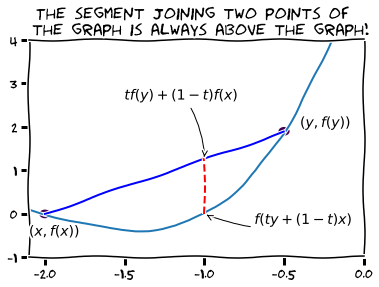
\includegraphics[width=0.5\linewidth]{convexFunction1.png} &
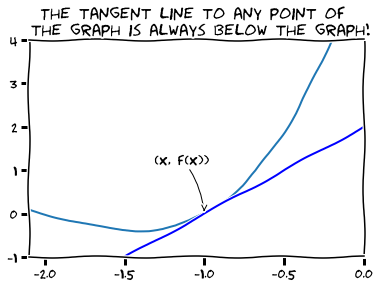
\includegraphics[width=0.5\linewidth]{convexFunction2.png}
\end{tabular}
\caption{Convex Functions.}
\label{figure:convexFunction}
\end{figure}
If instead we have $f\big(\lambda \x + (1-\lambda)f(\y)\big) < \lambda f(\x) + (1-\lambda) f(\y)$ for $0<\lambda<1$, we say that the function is \emph{strictly convex}.  A function $f$ is said to be \emph{concave} (resp.~\emph{strictly concave}) if $-f$ is convex (resp.~strictly convex).
\end{definition}